\documentclass[12pt]{article}
    \title{\vspace{-50pt}\textbf{\underline{CAP6635 Assignment 3 - Explanations}}}
    \author{William L. Thomson Jr.}
    \date{Spring Semester 2024}

	\usepackage{amssymb}
    \usepackage{enumitem}
    \usepackage{float}
    \usepackage{hyperref}
    \usepackage{graphicx}
    \usepackage[T1]{fontenc}
    \usepackage{titlesec}
    \usepackage[tmargin=1in,lmargin=1in,rmargin=1in]{geometry}

\begin{document}

\maketitle

\vspace{-1.75em}

\begin{figure}[H]
\begin{center}
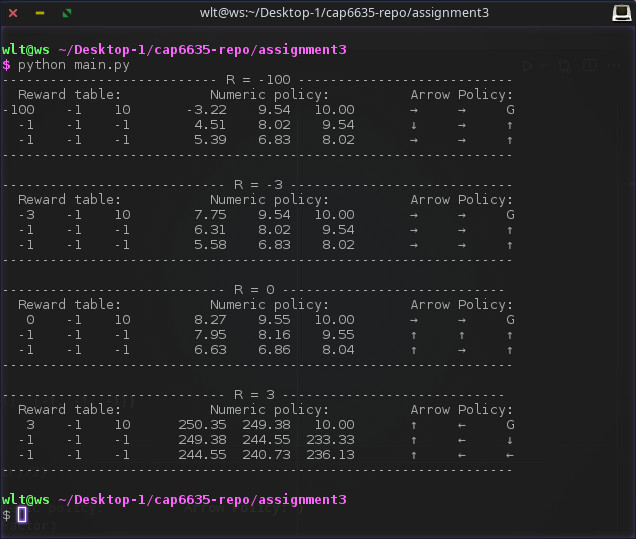
\includegraphics[scale=0.75]{screenshot}
\caption{Screenshot of policies for different values of R}
\label{figure1}
\end{center}
\end{figure}

\begin{description}[leftmargin=0cm]
	\item[When R = -100] \hfill \break
		With this heavy penalty, the state almost acts like a fire pit, or penalty termination
		rather than goal termination. For any movements within that state, you want to get out
		out of that miserable state as soon as possible, and given the +10 reward 2 states away
		the best action there is to go right to the goal/terminal state. The same for the top
		middle state, it surely does not want to go left to -100 vs right to +10, so it goes
		right. All other states, seek to avoid the top left corner and instead head
		to the goal, the top left. The utility values are increasing along the diagonal from
		the bottom left corner, to the top right goal/terminal state.
		
		The outlier is the middle left most state, below the top left heavy penalty state.
		Because sometimes actions in that state can go up, to the heavy penalty state,
		there is preference to not even get near or allow that and go down instead. By going
		down, it cannot go backward so it eliminates that chance, rather than going right
		which has a higher utility, than going down, but has a chance of going up, so best
		to just avoid entirely.
		
		Numerically, the heavy penalty state is the only one that remains with a negative
		utility even after all states utilities have converged. Again, further reflecting
		the undesirable state, and a result of it being -100 with all others being -1.
		Though the impact of that heavily penalty is not reflected in other nearby states,
		like the one to the right, which has the same utility as the state beneath
		goal/terminal state, reflecting that the heavy penalty state to the left does not
		impact its utility value being next to the goal.

	\item[When R = -3] \hfill \break
		With this more moderate penalty, things change from the heavy penalty. Even with the
		desire to leave that state, the action is similar to all other states, head for the
		goal as soon as possible. For this value, again across the diagonal, there is increasing
		utility values as you get closer to the goal, reflecting the higher probability
		of reaching the goal with a higher reward. All states to the left of the goal state,
		head right towards the goal, and states beneath the goal/terminal state simply head
		up to reach the goal.
		
		Unlike the previous case, there are no outliers, and since the penalty of the top
		left is not so great, the state beneath it will sometimes choose to go up, and
		because of such, the optimal action goes right towards the goal, despite the risk
		of ending up in the negative utility state sometimes, unlike with R = -100.


	\item[When R = 0] \hfill \break
		This is the most straight forward one, with the top left having a slightly lower
		or neutral reward when compared to others. Because of such, this one ends up a
		simple head for the goal/terminal state. With the top row heading straight for
		the goal, and all rows beneath heading straight up to one of those goal/termination
		bound states, or directly to the goal for states beneath, with some ties along the way
		numerically.
		
		Once again, across the diagonal from bottom left to top right, values were increasing
		with only a slight final variance between the top left and the bottom right, despite
		difference in initial reward values being greater.
		
		\textbf{Note:} There was an outlier in the arrow policy where it did not match the
		numeric, some bug in the arrow policy creation from numeric, despite storing optimal
		action with all utility values, which worked in every other state for all R values,
		except for this one, with the middle state, pointing right vs up, per numeric policy.
		
		
	\item[When R = +3] \hfill \break
		This one is most interesting, the introduction of a state with a positive reward, while
		all others were negative, aside from the goal/terminal state. Despite the goal/terminal
		state having a higher initial reward, due the math from the value iteration algorithm
		all other states end up with higher utility values than the goal, including the state
		that had the positive reward value. This deviated from the utility of any state being
		bounded by $\pm R_{max}$, as all states utilities ended up substantially > $R_{max}$
		
		In fact, that positive reward ended up being so great, and with the goal state reward
		never changing, all others ended up much higher than the initial goal/utility state.
		It essentially hijacks the goal/terminal state, and all other states head for the 
		top left and literally avoid the goal/terminal state, even for states next to the
		goal/terminal state.
		
		Even more interesting, because all other values outside the top left state were
		negative rewards the action in that state was such that it chose to never leave that
		state. Instead, it would rather bash into the wall over and over and still gain more
		than if it ever attempted to head to the goal/terminal state. However, since the
		goal/terminal state is present, the optimal action ended up being going up in that
		state vs left. That preference is difficult to explain since left would prevent it
		from going backwards to the lowest utility, the goal/terminal state. By going up,
		there is still the chance that sometimes it could go right, which it cannot, if it
		went left instead of up.
		
		Finally, the most interesting state here, is the one right below the goal/terminal
		state, which makes it act like it did when there was a heavy penalty reward, like
		in the R = -100 case, where all states wanted to stay away, and the state beneath
		goal/terminal state, just like in R = -100, the state below the top left, it would
		rather go down, than left, or in R = -100 case right, on the chance that it might
		end up in that heavy penalty state, which in this case is the goal/terminal state.
		
		This shows this method for a reward system is not practical, as it will entirely
		avoid the intended goal/terminal state, and choose another, as a result of the
		algorithm, whereas, the other three values of R, produced policies that from any
		state would take you to the goal/terminal state. This value will only take all
		to a state of perpetual head banging, good for people into heavy metal and rock,
		but bad for robots, or ever reaching any intended goal/terminal state.
		

\end{description}
\end{document}

